% questions.tex —— 2013 年·安徽卷·文科 · 题目内容片段（无答案）
% 由 tools/generate_projects.py 依来源总账自 2013/2013_数学真题_安徽文_试题.md 生成，勿手改（改源 MD 后重跑）

\gkpart{一、选择题}

\begin{question}
\gkti{1}设 $\mathrm i$ 是虚数单位，若复数 $a-\dfrac{10}{3-\mathrm i}$（$a\in\mathbf R$）是纯虚数，则 $a$ 的值为\mbox{（　　）}

（A）$-3$；（B）$-1$；（C）$1$；（D）$3$。

\end{question}
\begin{question}
\gkti{2}已知 $A=\{x\mid x+1>0\}$，$B=\{-2,-1,0,1\}$，则 $\complement_{\mathbf R}A\cap B=$\mbox{（　　）}

（A）$\{-2,-1\}$；（B）$\{-2\}$；（C）$\{-1,0,1\}$；（D）$\{0,1\}$。

\Needspace{0.4\textheight}
\end{question}
\begin{question}
\gkti{3}如图所示，程序框图（算法流程图）的输出结果是\mbox{（　　）}
\nopagebreak[4]
\begin{center}% 2013 年安徽卷文科第 3 题：输出 s 的程序框图（算法流程图）。
% 来源 PDF：普通高考/2013/2013安徽文.pdf，第 1 页（印面 785）左栏。
% 流程：开始 → s=0,n=2 → n<8? 是：s=s+1/n，n=n+2，回到判断；否：输出 s → 结束。
\begin{tikzpicture}[semithick, >=Stealth, font=\small,
  block/.style={draw, minimum width=2.9cm, minimum height=0.62cm, align=center},
  dec/.style={draw, diamond, aspect=2.5, inner sep=1pt, align=center},
  term/.style={draw, rounded corners=6pt, minimum width=1.4cm, minimum height=0.52cm},
  io/.style={draw, trapezium, trapezium left angle=70, trapezium right angle=110,
             minimum width=2.3cm, minimum height=0.62cm},
  arr/.style={->}]
  \node (start) [term] at (0,0) {开始};
  \node (init)  [block] at (0,-1.05) {$s=0,\ n=2$};
  \node (dec)   [dec]  at (0,-2.55) {$n<8$?};
  \node (body)  [block] at (0,-4.0) {$s=s+\dfrac1n$};
  \node (inc)   [block] at (0,-5.3) {$n=n+2$};
  \node (out)   [io]   at (3.2,-4.0) {输出 $s$};
  \node (end)   [term] at (3.2,-5.3) {结束};
  \draw[arr] (start) -- (init);
  \draw[arr] (init) -- (dec);
  \draw[arr] (dec) -- node[left, xshift=-1pt] {是} (body);
  \draw[arr] (body) -- (inc);
  \draw[arr] (dec.east) -- node[above] {否} (3.2,-2.55) -- (out.north);
  \draw[arr] (out) -- (end);
  % 是分支的回路：n=n+2 后向左、向上，再向右汇入判断框上方的流程线
  \draw[arr] (inc.west) -- (-2.0,-5.3) -- (-2.0,-1.8) -- (0,-1.8);
\end{tikzpicture}
\end{center}
\nopagebreak[4]
（A）$\dfrac34$；（B）$\dfrac16$；（C）$\dfrac{11}{12}$；（D）$\dfrac{25}{24}$。

\end{question}
\begin{question}
\gkti{4}“$(2x-1)x=0$”是“$x=0$”的\mbox{（　　）}

（A）充分不必要条件；（B）必要不充分条件；（C）充分必要条件；（D）既不充分也不必要条件。

\end{question}
\begin{question}
\gkti{5}若某公司从五位大学毕业生甲、乙、丙、丁、戊中录用三人，这五人被录用的机会均等，则甲或乙被录用的概率为\mbox{（　　）}

（A）$\dfrac23$；（B）$\dfrac25$；（C）$\dfrac35$；（D）$\dfrac9{10}$。

\end{question}
\begin{question}
\gkti{6}直线 $x+2y-5+\sqrt5=0$ 被圆 $x^2+y^2-2x-4y=0$ 截得的弦长为\mbox{（　　）}

（A）$1$；（B）$2$；（C）$4$；（D）$4\sqrt6$。

\end{question}
\begin{question}
\gkti{7}设 $S_n$ 为等差数列 $\{a_n\}$ 的前 $n$ 项和，$S_8=4a_3$，$a_7=-2$，则 $a_9=$\mbox{（　　）}

（A）$-6$；（B）$-4$；（C）$-2$；（D）$2$。

\Needspace{0.4\textheight}
\end{question}
\begin{question}
\gkti{8}函数 $y=f(x)$ 的图象如图所示，在区间 $[a,b]$ 上可找到 $n$（$n\geqslant2$）个不同的数 $x_1$，$x_2$，$\cdots$，$x_n$，使得 $\dfrac{f(x_1)}{x_1}=\dfrac{f(x_2)}{x_2}=\cdots=\dfrac{f(x_n)}{x_n}$，则 $n$ 的取值范围为\mbox{（　　）}
\nopagebreak[4]
\begin{center}% 2013 年安徽卷文科第 8 题：函数 y=f(x) 在 [a,b] 上的图象。
% 来源 PDF：普通高考/2013/2013安徽文.pdf，第 1 页（印面 785）中栏上部。
% 曲线自 (a,0) 陡升，经一个较高的极大值、一个正的极小值、一个较低的极大值，
% 最后降回 (b,0)；全部位于 x 轴上方（端点除外）。
\begin{tikzpicture}[semithick, >=Stealth, font=\small, x=0.95cm, y=0.95cm]
  \draw[->] (-0.35,0) -- (7.3,0) node[below right] {$x$};
  \draw[->] (0,-0.4) -- (0,3.3) node[right] {$y$};
  \node[below left] at (0,0) {$O$};
  \draw[thick] (1,0)
    .. controls (1.03,1.0) and (1.18,2.55) .. (1.62,2.60)
    .. controls (2.0,2.64) and (2.55,1.35) .. (3.05,0.98)
    .. controls (3.45,0.76) and (3.75,1.10) .. (4.15,1.28)
    .. controls (4.45,1.40) and (4.62,1.25) .. (4.95,1.02)
    .. controls (5.35,0.70) and (6.42,0.20) .. (6.45,0);
  \draw (1,0) -- (1,-0.06) node[below] {$a$};
  \draw (6.45,0) -- (6.45,-0.06) node[below] {$b$};
\end{tikzpicture}
\end{center}
\nopagebreak[4]
（A）$\{2,3\}$；（B）$\{2,3,4\}$；（C）$\{3,4\}$；（D）$\{3,4,5\}$。

\end{question}
\begin{question}
\gkti{9}设 $\triangle ABC$ 的内角 $A$，$B$，$C$ 所对边的长分别为 $a$，$b$，$c$，若 $b+c=2a$，$3\sin A=5\sin B$，则角 $C=$\mbox{（　　）}

（A）$\dfrac\pi3$；（B）$\dfrac{2\pi}3$；（C）$\dfrac{3\pi}4$；（D）$\dfrac{5\pi}6$。

\end{question}
\begin{question}
\gkti{10}已知函数 $f(x)=x^3+ax^2+bx+c$ 有两个极值点 $x_1$，$x_2$，若 $f(x_1)=x_1<x_2$，则关于 $x$ 的方程 $3(f(x))^2+2af(x)+b=0$ 的不同实根个数为\mbox{（　　）}

（A）$3$；（B）$4$；（C）$5$；（D）$6$。

\end{question}
\gkpart{二、填空题}

\begin{question}
\gkti{11}函数 $y=\ln\left(1+\dfrac1x\right)+\sqrt{1-x^2}$ 的定义域为\gkblank{}。

\end{question}
\begin{question}
\gkti{12}若非负变量 $x$，$y$ 满足约束条件 $\begin{cases}x-y\geqslant-1,\\ x+2y\leqslant4,\end{cases}$ 则 $x+y$ 的最大值为\gkblank{}。

\end{question}
\begin{question}
\gkti{13}若非零向量 $\boldsymbol a$，$\boldsymbol b$ 满足 $|\boldsymbol a|=3|\boldsymbol b|=|\boldsymbol a+2\boldsymbol b|$，则 $\boldsymbol a$ 与 $\boldsymbol b$ 夹角的余弦值为\gkblank{}。

\end{question}
\begin{question}
\gkti{14}定义在 $\mathbf R$ 上的函数 $f(x)$ 满足 $f(x+1)=2f(x)$。若当 $0\leqslant x\leqslant1$ 时，$f(x)=x(1-x)$，则当 $-1\leqslant x\leqslant0$ 时，$f(x)=$\gkblank{}。

\Needspace{0.4\textheight}
\end{question}
\begin{question}
\gkti{15}如图，正方体 $ABCD\text{-}A_1B_1C_1D_1$ 的棱长为 $1$，$P$ 为 $BC$ 中点，$Q$ 为线段 $CC_1$ 上的动点，过 $A$、$P$、$Q$ 的平面截该正方体所得的截面记为 $S$，则下列命题正确的是\gkblank{}。（写出所有正确命题的编号）
\nopagebreak[4]
\begin{center}% 2013 年安徽卷文科第 15 题：正方体 ABCD-A1B1C1D1，P 为 BC 中点，Q 在 CC1 上。
% 来源 PDF：普通高考/2013/2013安徽文.pdf，第 1 页（印面 785）中栏下部。
% 斜二测投影：screen(x,y,z) = (2.2x + 1.0y, 0.62y + 2.2z)，棱长 1。
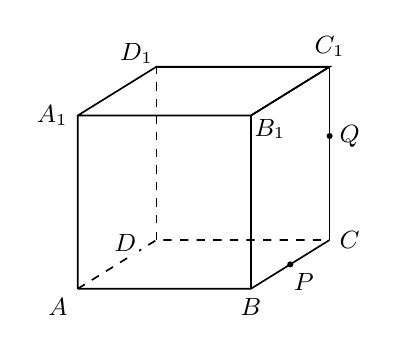
\begin{tikzpicture}[semithick, font=\small]
  \coordinate (A)  at (0,0);
  \coordinate (B)  at (2.2,0);
  \coordinate (C)  at (3.2,0.62);
  \coordinate (D)  at (1.0,0.62);
  \coordinate (A1) at (0,2.2);
  \coordinate (B1) at (2.2,2.2);
  \coordinate (C1) at (3.2,2.82);
  \coordinate (D1) at (1.0,2.82);
  \coordinate (P)  at (2.7,0.31);
  \coordinate (Q)  at (3.2,1.94);
  % 可见棱
  \draw (A) -- (B) -- (C);
  \draw (A) -- (A1) -- (B1) -- (C1) -- (D1) -- (A1);
  \draw (B) -- (B1);
  \draw (C) -- (C1);
  \draw (B1) -- (C1);
  \draw (C1) -- (D1);
  % 被遮挡的棱
  \draw[dashed] (A) -- (D) -- (C);
  \draw[dashed] (D) -- (D1);
  % 点 P、Q
  \fill (P) circle (1.1pt);
  \fill (Q) circle (1.1pt);
  % 标注
  \node[below left] at (A) {$A$};
  \node[below] at (B) {$B$};
  \node[right] at (C) {$C$};
  \node[left=6pt, yshift=-1pt, fill=white, inner sep=1pt] at (D) {$D$};
  \node[left] at (A1) {$A_1$};
  \node[below right, inner sep=1pt] at (B1) {$B_1$};
  \node[above] at (C1) {$C_1$};
  \node[above left, inner sep=1pt] at (D1) {$D_1$};
  \node[below right, yshift=-2pt, inner sep=1pt] at (P) {$P$};
  \node[right] at (Q) {$Q$};
\end{tikzpicture}
\end{center}
\nopagebreak[4]
\noindent ① 当 $0<CQ<\dfrac12$ 时，$S$ 为四边形；

\noindent ② 当 $CQ=\dfrac12$ 时，$S$ 为等腰梯形；

\noindent ③ 当 $CQ=\dfrac34$ 时，$S$ 与 $C_1D_1$ 交点 $R$ 满足 $C_1R=\dfrac13$；

\noindent ④ 当 $\dfrac34<CQ<1$ 时，$S$ 为六边形；

\noindent ⑤ 当 $CQ=1$ 时，$S$ 的面积为 $\dfrac{\sqrt6}2$。

\end{question}
\gkpart{三、解答题}

\begin{question}
\gkti{16}设函数 $f(x)=\sin x+\sin\left(x+\dfrac\pi3\right)$。

（1） 求 $f(x)$ 的最小值，并求使 $f(x)$ 取得最小值的 $x$ 的集合；

（2） 不画图，说明函数 $y=f(x)$ 的图象可由 $y=\sin x$ 的图象经过怎样的变化得到。

\Needspace{0.4\textheight}
\end{question}
\begin{question}
\gkti{17}为调查甲、乙两校高三年级学生某次联考数学成绩情况，用简单随机抽样，从这两校中各抽取 $30$ 名高三年级学生，以他们的数学成绩（百分制）作为样本，样本数据的茎叶图如图：
\nopagebreak[4]
\begin{center}% 2013 年安徽卷文科第 17 题：甲、乙两校各 30 名学生数学成绩的茎叶图。
% 来源 PDF：普通高考/2013/2013安徽文.pdf，第 1 页（印面 785）右栏。
% 茎为十位数字 4—9；甲校叶置左、乙校叶置右，逐位照录原图（未重新排序）。
\begin{tikzpicture}[font=\small, x=1cm, y=1cm]
  % 表头
  \node at (-0.7,0.52) {甲};
  \node at (2.35,0.52) {乙};
  \draw (-2.5,0.3) -- (3.9,0.3);
  % 双竖线与茎
  \draw (0.28,0.22) -- (0.28,-2.42);
  \draw (0.98,0.22) -- (0.98,-2.42);
  % 各行：茎 4—9
  \foreach \stem/\y in {4/0, 5/-0.44, 6/-0.88, 7/-1.32, 8/-1.76, 9/-2.2} {
    \node at (0.63,\y) {$\stem$};
  }
  % 甲校叶（右对齐）
  \node[anchor=east] at (0.17,0)    {$7$};
  \node[anchor=east] at (0.17,-0.44){$5\ 3\ 3\ 2$};
  \node[anchor=east] at (0.17,-0.88){$5\ 5\ 4\ 3\ 3\ 3\ 1\ 0\ 0$};
  \node[anchor=east] at (0.17,-1.32){$8\ 6\ 6\ 2\ 2\ 1\ 1\ 0\ 0$};
  \node[anchor=east] at (0.17,-1.76){$7\ 5\ 4\ 4\ 2$};
  \node[anchor=east] at (0.17,-2.2) {$2\ 0$};
  % 乙校叶（左对齐）
  \node[anchor=west] at (1.09,0)    {$5$};
  \node[anchor=west] at (1.09,-0.44){$3\ 3\ 8$};
  \node[anchor=west] at (1.09,-0.88){$0\ 0\ 0\ 1\ 1\ 2\ 2\ 3\ 3\ 5$};
  \node[anchor=west] at (1.09,-1.32){$0\ 0\ 2\ 2\ 2\ 3\ 3\ 6\ 6\ 9$};
  \node[anchor=west] at (1.09,-1.76){$1\ 1\ 5\ 5\ 8$};
  \node[anchor=west] at (1.09,-2.2) {$0$};
\end{tikzpicture}
\end{center}
\nopagebreak[4]
（1） 若甲校高三年级每位学生被抽取的概率为 $0.05$，求甲校高三年级学生总人数，并估计甲校高三年级这次联考数学成绩的及格率（$60$ 分及 $60$ 分以上为及格）；

（2） 设甲、乙两校高三年级学生这次联考数学平均成绩分别为 $\overline{x}_1$，$\overline{x}_2$，估计 $\overline{x}_1-\overline{x}_2$ 的值。

\Needspace{0.4\textheight}
\end{question}
\begin{question}
\gkti{18}如图，四棱锥 $P\text{-}ABCD$ 的底面 $ABCD$ 是边长为 $2$ 的菱形，$\angle BAD=60^\circ$。已知 $PB=PD=\sqrt2$，$PA=\sqrt6$。

（1） 证明：$PC\perp BD$；

（2） 若 $E$ 为 $PA$ 的中点，求三棱锥 $P\text{-}BCE$ 的体积。
\nopagebreak[4]
\begin{center}% 2013 年安徽卷文科第 18 题：四棱锥 P-ABCD，底面 ABCD 是菱形，E 为 PA 中点。
% 来源 PDF：普通高考/2013/2013安徽文.pdf，第 2 页（印面 786）左栏。
% 底面菱形按斜二测投影画出：A 左、B 前、C 右、D 后；D 与 PD 被遮挡。
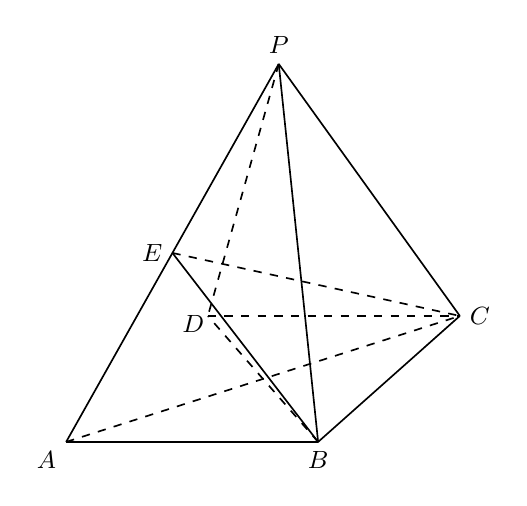
\begin{tikzpicture}[semithick, font=\small]
  \coordinate (A) at (0,0);
  \coordinate (B) at (3.2,0);
  \coordinate (C) at (5.0,1.6);
  \coordinate (D) at (1.8,1.6);
  \coordinate (P) at (2.7,4.8);
  \coordinate (E) at (1.35,2.4);
  % 可见棱
  \draw (P) -- (A);
  \draw (P) -- (B);
  \draw (P) -- (C);
  \draw (A) -- (B) -- (C);
  \draw (E) -- (B);
  % 被遮挡的棱与辅助线
  \draw[dashed] (P) -- (D);
  \draw[dashed] (D) -- (C);
  \draw[dashed] (A) -- (C);
  \draw[dashed] (B) -- (D);
  \draw[dashed] (E) -- (C);
  % 标注
  \node[above] at (P) {$P$};
  \node[below left] at (A) {$A$};
  \node[below] at (B) {$B$};
  \node[right] at (C) {$C$};
  \node[left, yshift=-3pt, fill=white, inner sep=1pt] at (D) {$D$};
  \node[left] at (E) {$E$};
\end{tikzpicture}
\end{center}
\nopagebreak[4]
\end{question}
\begin{question}
\gkti{19}设数列 $\{a_n\}$ 满足 $a_1=2$，$a_2+a_4=8$，且对任意 $n\in\mathbf N^*$，函数 $f(x)=(a_n-a_{n+1}+a_{n+2})x+a_{n+1}\cos x-a_{n+2}\sin x$ 满足 $f'\left(\dfrac\pi2\right)=0$。

（1） 求数列 $\{a_n\}$ 的通项公式；

（2） 若 $b_n=2\left(a_n+\dfrac1{2^{a_n}}\right)$，求数列 $\{b_n\}$ 的前 $n$ 项和 $S_n$。

\end{question}
\begin{question}
\gkti{20}设函数 $f(x)=ax-(1+a^2)x^2$，其中 $a>0$，区间 $I=\{x\mid f(x)>0\}$。

（1） 求 $I$ 的长度（注：区间 $(\alpha,\beta)$ 的长度定义为 $\beta-\alpha$）；

（2） 给定常数 $k\in(0,1)$，当 $1-k\leqslant a\leqslant1+k$ 时，求 $I$ 长度的最小值。

\end{question}
\begin{question}
\gkti{21}已知椭圆 $C:\dfrac{x^2}{a^2}+\dfrac{y^2}{b^2}=1$（$a>b>0$）的焦距为 $4$，且过点 $P(\sqrt2,\sqrt3)$。

（1） 求椭圆 $C$ 的方程；

（2） 设 $Q(x_0,y_0)$（$x_0y_0\neq0$）为椭圆 $C$ 上一点，过点 $Q$ 作 $x$ 轴的垂线，垂足为 $E$。取点 $A(0,2\sqrt2)$，连接 $AE$。过点 $A$ 作 $AE$ 的垂线交 $x$ 轴于点 $D$。点 $G$ 是点 $D$ 关于 $y$ 轴的对称点，作直线 $QG$，问这样作出的直线 $QG$ 是否与椭圆 $C$ 一定有唯一的公共点？并说明理由。

\end{question}